%File: formatting-instruction.tex
\documentclass[letterpaper]{article}
\usepackage{aaai}
\usepackage{times}
\usepackage{helvet}
\usepackage{algorithm}
\usepackage{algpseudocode}
\usepackage{courier}
\usepackage{graphicx}
\graphicspath{{./figure/}}
\frenchspacing
\setlength{\pdfpagewidth}{8.5in}
\setlength{\pdfpageheight}{11in}
\pdfinfo{
/Title (Multiple Object Tracking using Spatial Reasoning)
/Author (Xiaoyu Ge, Jochen Renz)}
\title{Multiple Object Tracking using Spatial Reasoning}
\author{Xiaoyu Ge \and Jochen Renz \\
Research School of Computer Science\\
The Australian National University \\
Canberra, Australia\\
\{xiaoyu.ge, jochen.renz\}@anu.edu.au
}
\setcounter{secnumdepth}{0}  
 \begin{document}


\section{Efficient Matching by Approximating Movement}\label{approxM}

To find out the best matchings, a straightforward approach is to enumerate all the possibilities. The search space is huge as there is a combinatorial number of potential matches between any two object sets. However, most matches can be avoided by searching through the corresponding objects only in a limited area. The area of the initial object should therefore cover all the objects in the subsequent scene that can be potentially matched to the initial object.  We use a circular region to represent this area. The circle's centre is located at the centroid of the initial object and the radius of the circle is the maximum shift of the centroid. The radius is calculated as $v \times t$ where $v$ is the maximum velocity of the object and $t$ is the time gap between the initial and subsequent scenes. This calculation ensures that the circle can adapt to different time gaps. We call this circle the $movement\,bounding\,circle$(MBC).  
\begin{figure}[h!]
\centering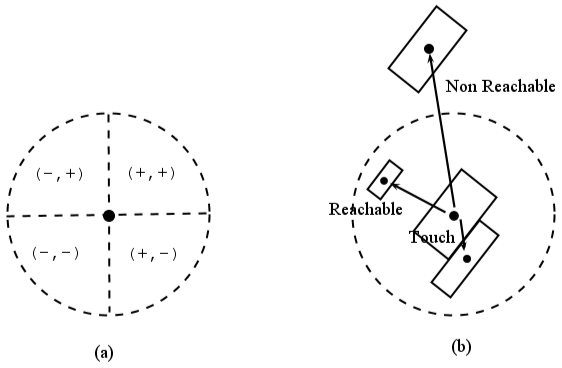
\includegraphics[scale=0.3]{quadrants.png}\caption{(a) The four quadrants of a MBC (b) Qualitative distance with respect to object A and its MBC}
\label{Quadrants}
\end{figure}

The relative distance between two objects can then be allocated to three meaningful classes, namely touch, reachable, and non-reachable (Figure \ref{Quadrants}.b). An object $o$ can touch another object $o^\prime$ at one of its contact sectors. $o^\prime$ is reachable by $o$ if $o^\prime$ is within the MBC of $o$ otherwise non-reachable. 

The MBC can be divided into four quadrants to further restrict the search area. A quadrant of an object is said to be active if the object is likely to be in that quadrant at the next time point, otherwise the quadrant is inactive. The search space can be reduced by first searching possible matches in the active quadrants, if there are no such matches, then searching in the other quadrants. Given a MBC $C$, the active quadrants are $C^{(i,j)}, i,j \in \{-, +, *\}$ where $(+,+)$, $(+,-)$, $(-,-)$, $(-,+)$ correspond to the top-right, top-left, bottom-left, bottom-right quadrants respectively (Figure \ref{Quadrants}.a). $(*, *)$ refers to an arbitrary quadrant. 

We can infer the active quadrants for an object by approximating the movement direction of the object, i.e. by estimating which of the quadrants the object is most likely to be in at the next time point. Object movement can be inferred from impact. Knowing the direction and the force of an impact, one can approximate the subsequent movements of the objects affected by the impact, directly or indirectly. When the impact information is not available, we can still approximate the movement by analysing structural properties, e.g. the stability of an object or a group of objects. An object is stable when it is supported and remains static. %An unstable object can have one of two possible motions, free fall if it is unsupported or fall to the side where there are no supports. %

We call the movement approximating problem we want to solve MQSR($\Theta$, \cal{R}, $M_{\cal{R}}$) where $\Theta$ is a set of objects in a spatial scenario and \cal{R} is a qualitative spatial representation of the objects. $M_{\cal{R}}$ is a reasoning model composed of a set of configurations written in the relations defined by \cal{R} by satisfying which the corresponding active quadrants of an object can be obtained. For each object in $\Theta$, we want to estimate the object's active quadrants by evaluating the object's spatial configurations against $M_{\cal{R}}$.

We demonstrate the movement approximation in the Angry Birds scenario where a bird hit usually comes from the left. We use $EGSR$ to represent the spatial configuration of a scenario. The model we use is mainly based on the stability analysis.

\cite{Ge2013} defined four kinds of supports that can make a solid rectangle stable and provided the corresponding GSR configurations. Our model $M$ contains all such stable configurations. Given each object, the model will evaluate the stability of the object by the configurations and return $C^{(*,-)}$ for the unstable objects.

A stable object may become unstable if it loses a support due to a bird hit. From the bird's trajectory, we can determine which object will be hit by the bird, and approximate the stability of the resulting scenario with the removal of that object.(Figure \ref{BirdImpact}). 

We can get a more restricted area, $C^{(+,-)}$ or $C^{(-,-)}$, by analysing the direction in which the object is falling. For example, a right / left leaning rectangle will fall to the right / left if there is no support at the right / left side, and the corresponding active quadrant is $C^{(+,-)}$ / $C^{(-, +)}$ (Figure \ref{QudrantsEstimation}). Here we illustrate how can we express the configurations described in the example using EGSR relations. We denote the left leaning and right leaning objects as $O^L$, $O^R$ respectively, and the MBC of an object $o$ is written as $C_{o}$. the two configurations can be expressed using EGSR relations:
\begin{enumerate}
\item Right-leaning: $\forall o^R_1\,:\, \exists o^*_2\,o^R_1 (A_5, *) o^*_2 \wedge\neg\exists o^*_3\,o^R_1 (A_6, *) o^*_3 \wedge\neg\exists o^*_4\,o^R_1 (A_7, *) o^*_4 \Rightarrow \, C_{o^A_1}^{(+,-)}$

\item Left-leaning: $\forall o^L_1\,:\, \exists o^*_2\,o^L_1 (A_5, *) o^*_2 \wedge\neg\exists o^*_3\,o^L_1 (A_3, *) o^*_3 \wedge\neg\exists o^*_4\,o^L_1 (A_4, *) o^*_4 \Rightarrow \, C_{o^L_1}^{(+,-)}$
\end{enumerate}
The model $M_{\cal{R}}$ contains all such configurations and can be replaced with any other model using $EGSR$ relations. We will show the model $M_{\cal{R}}$, although simple, is sufficient to solve the tracking problem in the evaluation part.  


\begin{figure}[h!]
\centering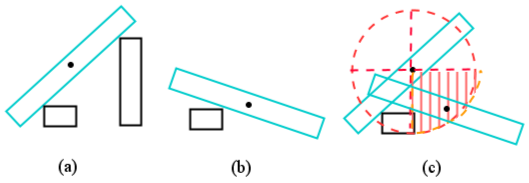
\includegraphics[scale=0.4]{QudrantsEstimation.png}\caption{(a) The right-leaning object (in cyan)  (b) a subsequent scene where the object falls to the right (c) The estimated active quadrant (shadowed area)}
\label{QudrantsEstimation}
\end{figure}


\begin{figure}[h!]
\centering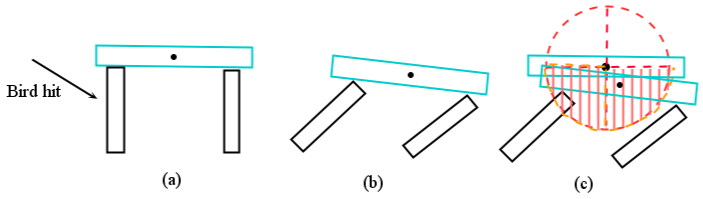
\includegraphics[scale=0.35]{BirdImpact.png}\caption{(a) The object in cyan is stable, and the impending impact is indicated by the arrow (b) A subsequent scene after the bird hit (c) The estimated active quadrant (shadowed area)}
\label{BirdImpact}
\end{figure}

\begin{figure}[h!]
\centering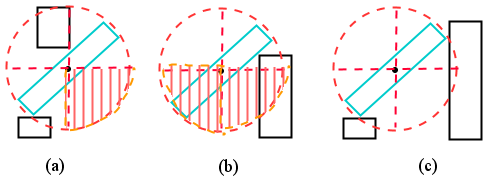
\includegraphics[scale=0.4]{ScenarioByRules.png}\caption{ The active quadrants of $o_1$ is (a) $C^{(+,-)}$ by satisfying the Right-leaning configuration (b) $C^{(*,-)}$ because there is no object contact $A_5$ of $o_1$ (c) No active quadrants as the object is stable}
\label{QudrantsEstimation}
\end{figure}



 \end{document}